% Stay on Task: mid-submission report. Build with: python mid_submission/build_report.py
\documentclass[10.5pt,a4paper]{article}

% ---------- fonts and page ----------
\usepackage[T1]{fontenc}
\usepackage[utf8]{inputenc}
\usepackage{XCharter}
\usepackage[scaled=0.86]{beramono}
\usepackage{microtype}
\usepackage[a4paper,top=24mm,bottom=22mm,left=21mm,right=21mm,headheight=14pt]{geometry}
\usepackage[table]{xcolor}
\usepackage{graphicx,booktabs,tabularx,array,multirow,makecell,enumitem,float,amsmath}
\usepackage[font=small,labelfont=bf,labelsep=period,skip=4pt]{caption}
\usepackage{fancyhdr,lastpage,titlesec,needspace}
\usepackage[most]{tcolorbox}
\usepackage[hidelinks]{hyperref}

% ---------- greyscale text ----------
\definecolor{ink}{gray}{0.0}
\definecolor{head}{gray}{0.12}
\definecolor{sub}{gray}{0.35}
\definecolor{rule}{gray}{0.55}
\definecolor{shade}{gray}{0.95}
\definecolor{rowshade}{gray}{0.965}
\color{ink}
\hypersetup{colorlinks=true,linkcolor=sub,urlcolor=head,citecolor=sub}

\titleformat{\section}{\needspace{9\baselineskip}\large\bfseries\color{head}}{\thesection}{0.6em}{}[{\color{rule}\titlerule[0.6pt]}]
\titleformat{\subsection}{\needspace{6\baselineskip}\normalsize\bfseries\itshape\color{head}}{\thesubsection}{0.6em}{}
\titlespacing*{\section}{0pt}{14pt}{6pt}
\titlespacing*{\subsection}{0pt}{9pt}{3pt}

\pagestyle{fancy}
\fancyhf{}
\fancyhead[L]{\small\itshape\color{sub}Stay on Task: mid-submission report}
\fancyhead[R]{\small\itshape\color{sub}LMA Group Project 2026}
\fancyfoot[C]{\small\color{sub}Page \thepage\ of \pageref{LastPage}}
\renewcommand{\headrulewidth}{0.4pt}
\renewcommand{\headrule}{\hbox to\headwidth{\color{rule}\leaders\hrule height \headrulewidth\hfill}}
\fancypagestyle{plain}{\fancyhf{}\renewcommand{\headrulewidth}{0pt}\fancyfoot[C]{\small\color{sub}Page \thepage\ of \pageref{LastPage}}}

\setlist{itemsep=1.5pt,topsep=3pt,parsep=0pt,leftmargin=14pt}
\setlength{\parindent}{0pt}
\setlength{\parskip}{5pt}
\renewcommand{\arraystretch}{1.22}

\newcolumntype{Y}{>{\raggedright\arraybackslash}X}

\newcolumntype{P}[1]{>{\raggedright\arraybackslash}p{#1}}
\newcommand{\tablestyle}{\small\rowcolors{2}{rowshade}{white}}
\newcommand{\code}[1]{\texttt{#1}}
\newcommand{\pts}[1]{#1}

\begin{document}

% ---------- title ----------
\thispagestyle{plain}
\begin{center}
{\color{rule}\rule{\linewidth}{1.4pt}}\\[6pt]
{\small\color{sub}\textsc{LMA Group Project 2026 \enspace·\enspace Mid-submission report \enspace·\enspace 30 October 2026}}\\[8pt]
{\LARGE\bfseries\color{head} Stay on Task: Can a small classifier\\[2pt] correct local agents' drift?}\\[11pt]
\begin{tabular}{cccc}
\textbf{Shuban Biswas} & \textbf{Ch Pavan Harshit} & \textbf{Swayam Goyal} & \textbf{Aaditya Sharma}\\
{\small 2024111017} & {\small 2025701057} & {\small 2024111012} & {\small 2019113009}
\end{tabular}\\[7pt]
{\small Team Stay on Task \enspace·\enspace Code, data and results: \url{https://github.com/ch-pavan/lma-grp-project/tree/main}}\\[4pt]
{\color{rule}\rule{\linewidth}{0.6pt}}
\end{center}

\begin{tcolorbox}[colback=shade,colframe=rule,boxrule=0.6pt,arc=1pt,left=8pt,right=8pt,top=5pt,bottom=5pt,fontupper=\small]
\textbf{Abstract.} Small agents that run locally and act through tools often lose track of a request, make up values, or claim work they never did. The usual guard is a language-model judge on every step, which is slow and costly. We test whether Laya, a 0.4B classifier finetuned for typed decisions, can judge an agent's steps better than a prompted 9B judge (the \emph{SLM judge}) given the same state, at a fraction of the cost.\par\smallskip
At mid-term we have built and run:
\begin{itemize}
  \item a planner, doer and judge harness on a cleaned BFCL multi-turn split
  \item three baseline systems run in full on the test set, plus pilots of two more
  \item recorded runs of three agent models
  \item labels for every validation step, with a 200-step annotation check
  \item two finetuned Laya heads
\end{itemize}
\smallskip
On validation, finetuned Laya beats the SLM judge at catching bad tool calls (F1 0.59 against 0.24, AUROC 0.91). It is also better at telling whether a turn is finished (F1 0.53 against 0.41). Each Laya check costs one forward pass, where the SLM judge writes about 1,500 to 2,400 tokens. The proposal's primary bar is a gain of 9 F1 points on the mean of off-track and false-claim F1. On validation the gap is only $-1.0$ to $+2.0$, because false claims are too rare to measure there and Laya has no false-claim head yet. The plan to the final submission therefore focuses on test passes sized for false claims, a false-claim head, and the test-set evaluation.
\end{tcolorbox}

{\small\tableofcontents}
\vspace{2pt}{\color{rule}\rule{\linewidth}{0.4pt}}

% =====================================================================
\section{Introduction}

\textbf{Problem.} The target user wants an agent that runs on their own machine, private and cheap, and acts on files, messages, posts, bookings and trading accounts. Small local models drift partway through such tasks in four ways:
\begin{itemize}
  \item they lose track of the request
  \item they fill in values nobody gave
  \item they report success after a failed call
  \item they make changes nobody asked for
\end{itemize}
A large judge on every step is too slow, and a small model judging itself is weak.

\textbf{Research question.} Can a finetuned small classifier, given the same state as an SLM judge, detect off-track steps and false claims better than that judge? And what does a system built around it do to task accuracy and cost?

\begin{table}[H]
\centering\tablestyle
\caption{Hypothesis and falsification, as in the proposal.}\label{tab:hyp}
\begin{tabularx}{\linewidth}{P{0.42\linewidth}Y}
\toprule
\rowcolor{white}\textbf{Claim} & \textbf{Falsified if} \\
\midrule
\textbf{Primary.} Finetuned Laya beats the SLM judge at catching off-track steps and false claims. & The gain in mean F1 (off track, false claim) is under 9 points, or its 95\% CI includes zero. A gain of 5 to 9 points is reported but does not confirm the hypothesis. \\
\textbf{Task.} Our system completes more tasks than no judge and about as many as the SLM-judge system, for a fraction of its judge tokens. & Tested only if the primary holds. It fails if the system does not beat no judge with a CI above zero, or if the lower end of its 95\% CI against the SLM-judge system is more than 5 points down. \\
\bottomrule
\end{tabularx}
\end{table}

\textbf{Key findings at mid-term.}
\begin{itemize}
  \item \textbf{Laya is a much better step checker than the SLM judge offline,} at near-zero cost (Section~\ref{sec:laya}).
  \item \textbf{A judge of single steps cannot see omissions,} which are about half of all failures, so we added a check at the end of each turn (Section~\ref{sec:agent}).
  \item \textbf{Block-and-warn corrections do not help even with a perfect judge,} and they hurt with the SLM judge. Only rollback plus the turn-end check moved task accuracy (Section~\ref{sec:ablations}).
  \item \textbf{The annotation passes the proposal's agreement bar} after one guide rewrite (Section~\ref{sec:annot}).
  \item \textbf{The primary metric cannot be measured on validation yet,} because there are too few false claims and Laya has no false-claim head. The test passes are sized for it (Section~\ref{sec:challenges}).
\end{itemize}

% =====================================================================
\section{Team and roles}

Every member worked across design, experiments and writing. Table~\ref{tab:roles} gives each person's main ownership.

\begin{table}[H]
\centering\tablestyle
\caption{Roles and main work.}\label{tab:roles}
\begin{tabularx}{\linewidth}{P{0.15\linewidth}P{0.16\linewidth}Y}
\toprule
\rowcolor{white}\textbf{Member} & \textbf{Role} & \textbf{Main work} \\
\midrule
\textbf{Swayam Goyal} & Annotation (Annotator A) & Annotated every validation step (1,277 calls, 495 turn ends) under guides v1 and v2, and the 200 check steps under v3. Rewrote the annotation guide (v3) from the check results, built the fresh check sample, wrote this report. \\
\textbf{Aaditya Sharma} & Annotation (Annotator B) & Annotated every validation step under guides v1 and v2, and the 200 check steps under v3. Analysed where the annotations differ from the checkers by error type; reviewed the guide and the proposal. \\
\textbf{Ch Pavan Harshit} & Checking, agent runs, Laya & Checker on the 200-step annotation check, adjudicating with Shuban. Ran the Qwen3.5 9B agent on Turing, finetuned Laya's two heads, ran the live checks and the primary-metric analysis. \\
\textbf{Shuban Biswas} & Checking, harness, baselines & Checker on the annotation check, adjudicating with Pavan. Built the harness and the replay oracle; ran the Qwen3 8B and Qwen3.5 4B baselines on BFCL test and AgentDojo, the correction-action study, and the offline scorer for off-the-shelf judges. \\
\bottomrule
\end{tabularx}
\end{table}

All four of us wrote and revised the proposal.

% =====================================================================
\section{Approach}\label{sec:approach}

\textbf{Agent.} For each user turn, a planner writes a short plan and a doer carries out the steps through tool calls. A judge checks each step before it runs, so a flagged call never executes. Both agent roles use Qwen3.5 9B (4-bit AWQ, reasoning off) served with vLLM.

\begin{figure}[H]
\centering
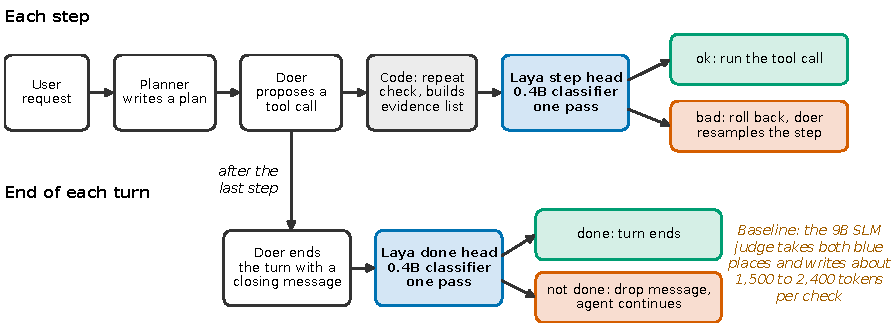
\includegraphics[width=\linewidth]{figs/fig1_system.pdf}
\caption{Our system. The blue boxes are the two Laya checks. In the baseline, the 9B SLM judge sits in both places and reasons before each answer.}\label{fig:system}
\end{figure}

\textbf{State given to the step judge.} The Laya step head and the SLM judge get the same input. Code builds it, up to 1,024 tokens:
\begin{itemize}
  \item the proposed call or closing message, placed first
  \item the current and earlier user requests
  \item the turn plan
  \item the last three calls, with their outputs cut short
  \item an \emph{evidence list}: for every argument value, where it appears (request, tool output, tool docs, environment, composed, arithmetic, or nowhere)
\end{itemize}
The done check instead gets the closing message, the user requests, and every call of the turn with its output cut short.

\textbf{Questions.} Code settles what needs no model: an exact repeat of a failed call. Laya answers typed questions, each with a fixed set of options and a confidence:
\begin{itemize}
  \item \textbf{Step head, on every tool call:} is this a bad step? Bad covers three cases:
  \begin{itemize}
    \item off track: the turn can no longer pass
    \item an unneeded irreversible call
    \item a made-up value on an irreversible call
  \end{itemize}
  \item \textbf{Done head, at every turn end:} is the latest request really finished, done or not done? A typed head (done, missing action, should ask the user, unsupported claim) is planned.
\end{itemize}

\textbf{Actions.} A bad step is rolled back and the doer resamples it, at most twice. A ``not done'' answer drops the closing message and tells the agent that part of the request may be unfinished, at most twice per turn.

% =====================================================================
\section{Progress against the proposal}

\begin{table}[H]
\centering\tablestyle
\caption{Status of each proposal item at mid-submission.}\label{tab:progress}
\begin{tabularx}{\linewidth}{P{0.36\linewidth}Y}
\toprule
\rowcolor{white}\textbf{Proposal item} & \textbf{Status} \\
\midrule
Harness: planner, doer, judge, fixed actions, rollback & \textbf{Done.} 20-step cap per turn. Correction modes: block and warn, rollback, deep rollback, vote of 3, done check. \\
BFCL multi-turn, cleaned, split by scenario, empty-turn check & \textbf{Done.} 74 train, 15 validation, 100 test scenarios; 11 unsound scenarios dropped. Gold replay passes 755 of 756 tasks. \\
AgentDojo benign tasks as an outside check & \textbf{Done} for no judge, rules and the SLM judge on the Qwen3 8B agent (97 tasks $\times$ 3 runs). \\
Natural agent runs for training & \textbf{Done.} Qwen3.5 9B: 888 train and 120 validation tasks. Qwen3 8B: 356 tasks. \\
Directed runs with a 32B model & \textbf{Dropped} (Section~\ref{sec:changes}). Training pools natural mistakes from two agent models (Qwen3.5 9B and Qwen3 8B). \\
Baselines: no judge, rules, SLM judge, Laya as is, Granite Guardian & \textbf{Done on test} with the Qwen3 8B agent for no judge, rules and the SLM judge (1,200 runs each). Laya as is was stopped after 133 runs and Granite Guardian ran as a 20-task pilot, both because they block most steps (Section~\ref{sec:online}). \\
Offline judges: Kev, LettuceDetect and others & \textbf{Done on validation} (Section~\ref{sec:offline}). Still to run offline: Granite Guardian, Jev on the full set, and Gemma 4 12B as a stronger reference judge. \\
Finetuned Laya & \textbf{Done for two heads,} step and done (Section~\ref{sec:laya}). A false-claim head is planned. \\
Annotation check (revised proposal) & \textbf{Done on 200 validation steps,} guide rewritten once (Section~\ref{sec:annot}). \\
Test labels and the primary metric on test & \textbf{Not yet.} Starts after the GPU budget resets on 1 November. \\
Confidence-gated escalation to the SLM judge & \textbf{Not yet,} after the test labels. \\
\bottomrule
\end{tabularx}
\end{table}

% =====================================================================
\section{Datasets}

\subsection{Benchmarks}
\textbf{BFCL multi-turn} (gorilla commit \code{6ea5797}):
\begin{itemize}
  \item \textbf{Size.} 200 scenarios in four versions: base, missing parameter, missing function and long context.
  \item \textbf{Domains.} Eight simulated apps: files, messages, posts, tickets, travel, trading, car and maths.
  \item \textbf{Cleaning.} 11 scenarios with unsound answer keys are dropped.
  \item \textbf{Split by scenario.} 74 train, 15 validation, 100 test. The test scenarios are never used for training, tuning or prompt choice.
  \item \textbf{Pass rule.} BFCL's own state checker plus our empty-turn check: on a turn whose correct answer is to call nothing, any state change fails it.
\end{itemize}

\textbf{AgentDojo benign user tasks} (agentdojo 0.1.35, suites v1.2.2):
\begin{itemize}
  \item \textbf{Size.} 97 tasks across workspace, travel, banking and Slack, with no injections.
  \item \textbf{Pass rule.} Each task's own utility check.
  \item \textbf{Use.} Outside check on task accuracy only: no training or tuning on it.
\end{itemize}

\subsection{Recorded agent runs}
\begin{table}[H]
\centering\tablestyle
\caption{Recorded agent runs (in \code{runs/raw/} and \code{shuban\_findings/finetune\_data/}).}\label{tab:runs}
\begin{tabularx}{\linewidth}{Yrp{0.4\linewidth}}
\toprule
\rowcolor{white}\textbf{Run} & \textbf{Tasks} & \textbf{Steps} \\
\midrule
Qwen3.5 9B, validation, reasoning off & 120 & 1,277 calls, 495 turn ends \\
Qwen3.5 9B, validation, reasoning on & 120 & 776 calls, used in the step check's validation set \\
Qwen3.5 9B, train & 888 & 8,806 calls, 3,737 turn ends \\
Qwen3 8B, train and validation scenarios & 356 & 3,824 steps, plus 3,635 gold replay steps \\
\bottomrule
\end{tabularx}
\end{table}

\subsection{Labels and class balance}
A replay oracle labels every step automatically. After each call, it replays every order-preserving subset of the turn's reference calls (up to 8) as the rest of the turn. The first call after which no ending passes is off track.

\begin{table}[H]
\centering\tablestyle
\caption{Class balance of the automatic labels (Qwen3.5 9B runs).}\label{tab:balance}
\begin{tabularx}{\linewidth}{YP{0.14\linewidth}rr}
\toprule
\rowcolor{white}\textbf{Label} & \textbf{Unit} & \textbf{Validation} & \textbf{Train} \\
\midrule
Off track & tool call & 63 of 1,277 (4.9\%) & 221 of 8,806 (2.5\%) \\
False claim (success words while the state is wrong) & closing message & 50 of 495 (10.1\%) & 281 of 3,737 (7.5\%) \\
Turn not done (wrong end state, or a reference function never called) & turn end & 111 of 495 (22.4\%) & 672 of 3,737 (18.0\%) \\
\bottomrule
\end{tabularx}
\end{table}

\textbf{How we handle the imbalance.}
\begin{itemize}
  \item \textbf{Metrics:} we report per-class F1, precision, recall and AUROC, never accuracy.
  \item \textbf{Training:} finetunes use balanced class weights, and thresholds are chosen on held-out dev scenarios.
  \item \textbf{Turn-end label:} it is better balanced. Train alone gives 672 unfinished turns, above the proposal's Gate~1 of 300 per class.
\end{itemize}

\subsection{Annotation}
The two annotators labelled all 1,772 validation steps from a written guide, without seeing the oracle labels or the BFCL verdict:
\begin{itemize}
  \item \textbf{Swayam Goyal:} Annotator A
  \item \textbf{Aaditya Sharma:} Annotator B
\end{itemize}

What each step gets:
\begin{itemize}
  \item \textbf{Tool call, Q1:} on track or off track.
  \item \textbf{Tool call, Q2:} none, made-up value or false claim.
  \item \textbf{Turn end:} one typed answer, from done, missing action, should ask the user, and unsupported claim.
\end{itemize}

Section~\ref{sec:annot} gives the quality check of these annotations.

\subsection{Laya training sets}
\begin{table}[H]
\centering\tablestyle
\caption{Laya training sets, split by scenario.}\label{tab:layadata}
\begin{tabularx}{\linewidth}{P{0.2\linewidth}YYP{0.16\linewidth}}
\toprule
\rowcolor{white}\textbf{Head} & \textbf{Train} & \textbf{Dev (threshold, epoch)} & \textbf{Validation} \\
\midrule
Done check & 3,341 turn ends, 66 scenarios & 396 turn ends, 8 held-out train scenarios & 495 turn ends \\
Step check (9B and 8B steps pooled; validation also has the 9B reasoning-on run) & 8,847 calls, 408 bad & 1,975 calls, 55 bad & 2,427 calls, 186 bad \\
\bottomrule
\end{tabularx}
\end{table}

% =====================================================================
\section{Evaluation protocol}
\begin{itemize}
  \item \textbf{Detection, offline:} per-class F1, precision, recall and AUROC on recorded steps.
  \item \textbf{Primary metric:} the mean of off-track F1 and false-claim F1, computed against the annotations.
  \item \textbf{Task accuracy, online:} the share of tasks passing BFCL's checker plus the empty-turn check.
  \item \textbf{Cost:} judge tokens and seconds per task.
  \item \textbf{Confidence intervals:} 95\%, from a bootstrap over scenarios, never over tasks, since tasks from one scenario are correlated.
  \item \textbf{Comparing systems:} differences use a paired bootstrap on the same tasks. Secondary comparisons are Holm-corrected.
\end{itemize}

\begin{table}[H]
\centering\tablestyle
\caption{Systems compared.}\label{tab:systems}
\begin{tabularx}{\linewidth}{P{0.1\linewidth}Y}
\toprule
\rowcolor{white}\textbf{Code} & \textbf{System} \\
\midrule
S1 & \textbf{No judge:} the planner and doer alone. \\
S2 & \textbf{Plain rules:} a value with no evidence is made up; a success word with no successful call is a false claim; a call not in the plan is drift; every irreversible call asks the user. \\
S3 & \textbf{SLM judge:} the agent model as judge, reasoning on, given the same state and guide as Laya. \\
S4a / S4b & Laya typed-decisions 0.4B as is / Granite Guardian 3.2 3B A800M. \\
Ours & \textbf{Finetuned Laya:} step head and done head, with rollback and the done check. \\
Oracle & \textbf{Ceiling, not deployable:} flags exactly the steps the replay oracle marks as wrong. \\
\bottomrule
\end{tabularx}
\end{table}

% =====================================================================
\section{Baseline experiments}

\subsection{Choice of agent model}\label{sec:agent}
\begin{figure}[H]
\centering
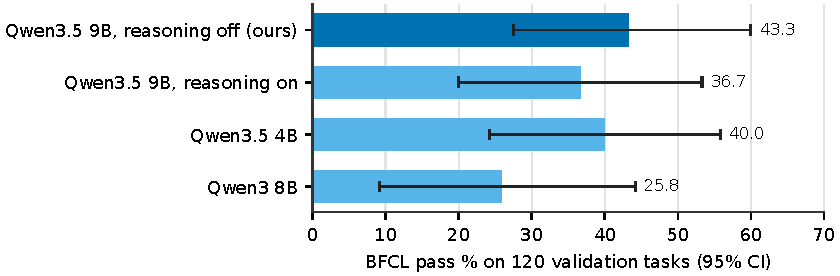
\includegraphics[width=0.72\linewidth]{figs/fig2_agents.pdf}
\caption{Agent models on the same 120 validation tasks. The Qwen3.5 9B with reasoning off is our agent.}\label{fig:agents}
\end{figure}

Figure~\ref{fig:agents} compares four agent setups:
\begin{itemize}
  \item \textbf{The model generation matters more than size.} Qwen3.5 4B passes 40.0\%, against 25.8\% for the older Qwen3 8B.
  \item \textbf{The 9B passes 43.3\%} on validation and 52.7\% [44.8, 60.5] on the 888 train tasks.
  \item \textbf{Reasoning on does not help.} It is 6.6 points lower and 2.5$\times$ slower, so the agent runs with reasoning off.
\end{itemize}

\begin{table}[H]
\centering\tablestyle
\caption{Why the 9B agent fails, by the first unfinished turn of each failed validation task.}\label{tab:failures}
\begin{tabularx}{\linewidth}{P{0.22\linewidth}Yr}
\toprule
\rowcolor{white}\textbf{Failure type} & \textbf{Meaning} & \textbf{Share} \\
\midrule
Stopped early & ended the turn with no success claim, often after a fixable error & 26.5\% \\
Wrong step & a call that made the right end state unreachable & 23.5\% \\
Acted instead of asking & changed state where the right move was to ask & 22.1\% \\
Claimed done & said it was done while the state was wrong & 17.6\% \\
Asked needlessly & asked the user although the request was answerable & 8.8\% \\
Checker only or step cap & & 1.5\% \\
\bottomrule
\end{tabularx}
\end{table}

About half of all failures are unfinished turns: stopped early, claimed done, or asked needlessly. A judge of the proposed step cannot see something that never happened. \textbf{This finding is why we added the done check at turn end.}

\subsection{Online judges on the test set}\label{sec:online}
\begin{table}[H]
\centering\tablestyle
\caption{Baselines on the BFCL test set: Qwen3 8B agent, 100 scenarios $\times$ 4 versions $\times$ 3 runs.}\label{tab:test}
\begin{tabularx}{\linewidth}{Yrlllr}
\toprule
\rowcolor{white}\textbf{System} & \textbf{Runs} & \textbf{Pass \% [95\% CI]} & \textbf{vs S1 [95\% CI]} & \textbf{s / task} & \textbf{Judge tok. / task} \\
\midrule
S1 no judge & 1,200 & 15.9 [11.7, 20.5] & & 93 & 0 \\
S2 plain rules & 1,200 & 7.6 [4.4, 11.2] & $-$8.3 [$-$11.8, $-$5.2] & 108 & 0 \\
S3 SLM judge & 1,200 & 17.4 [12.8, 22.3] & +1.5 [$-$0.6, +3.8] & 202 & 11.8k \\
S4a Laya as is & 133 (stopped) & 0 (upper bound 2.2) & & 336 & \\
S4b Granite Guardian & 20-task pilot & 0 & & & \\
\bottomrule
\end{tabularx}
\end{table}

\begin{figure}[H]
\centering
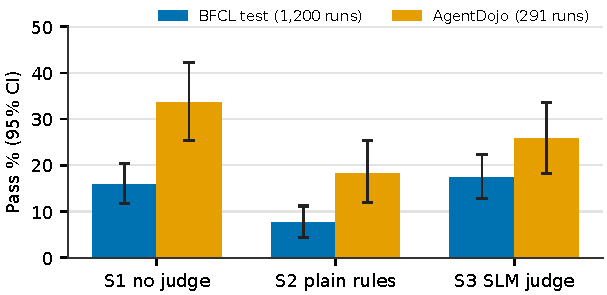
\includegraphics[width=0.66\linewidth]{figs/fig3_test_baselines.pdf}
\caption{Pass rates on BFCL test and AgentDojo, with 95\% confidence intervals.}\label{fig:test}
\end{figure}

\begin{itemize}
  \item \textbf{Rules hurt.} They block good calls: their made-up-value rule flags 1.8\% of gold calls.
  \item \textbf{Laya as is blocks almost everything.} It blocked 87.6\% of judged steps, so every run hit the step cap.
  \item \textbf{Granite Guardian also blocks almost everything.} It called all 169 calls it saw risky.
  \item \textbf{The SLM judge is the only system that does not hurt on BFCL.} It gains most on the missing-function (+7.3) and missing-parameter (+3.0) versions, but overall it is within noise, at twice the time per task.
  \item \textbf{Out of domain, the SLM judge loses.} On AgentDojo it drops 7.9 points (Figure~\ref{fig:test}).
\end{itemize}

\subsection{Off-the-shelf judges, offline}\label{sec:offline}
\begin{table}[H]
\centering\tablestyle
\caption{Primary score (mean F1 of off-track and false-claim steps) on the 1,772 validation steps of the 9B agent, against three label sources.}\label{tab:offline}
\begin{tabularx}{\linewidth}{Yccc}
\toprule
\rowcolor{white}\textbf{Judge} & \textbf{vs oracle} & \textbf{vs Swayam (A)} & \textbf{vs Aaditya (B)} \\
\midrule
Plain rules & 0.07 & 0.10 & 0.11 \\
Laya as is & 0.11 & 0.21 & 0.16 \\
Kev 0.8B & 0.15 & 0.12 & 0.07 \\
LettuceDetect (false claim only) & 0.18 & 0.22 & 0.15 \\
\bottomrule
\end{tabularx}
\end{table}

Every confidence interval overlaps, so no off-the-shelf judge is usable.

\textbf{Laya as is.} On the Qwen3 8B validation steps against the oracle labels, we swept it across 4 state formats, 8 question wordings, thresholds and a logistic head. Its AUROC stayed at 0.39 to 0.67. It keeps the start of its input and cuts the end, so on long states it never saw the step it was judging. Putting the step first fixed the cut but added no signal.

\textbf{Jev.} On the same steps, the hosted Jev classifier was the only off-the-shelf model with real signal, and only on closing messages (AUROC 0.81). \textbf{Finetuning is required.}

% =====================================================================
\section{Results: finetuned Laya}\label{sec:laya}

\subsection{Offline}
\begin{figure}[H]
\centering
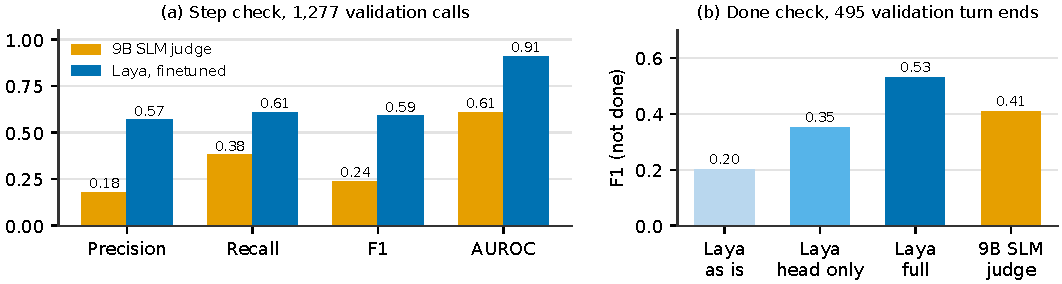
\includegraphics[width=\linewidth]{figs/fig4_offline_laya.pdf}
\caption{Finetuned Laya against the 9B SLM judge on the same validation steps. (a) Step check on tool calls. (b) Done check at turn end.}\label{fig:offlinelaya}
\end{figure}

Both heads use a full finetune with balanced class weights on one RTX 6000 Ada: 4 epochs and 16 minutes for the step check, and 4 epochs and 5 minutes for the done check.

\begin{table}[H]
\centering\tablestyle
\caption{Offline detection on validation: the step check on 1,277 calls (109 bad); the done check on 495 turn ends (positive class: not done).}\label{tab:offlinelaya}
\begin{tabularx}{\linewidth}{P{0.1\linewidth}Ycccc}
\toprule
\rowcolor{white}\textbf{Check} & \textbf{Checker} & \textbf{Precision} & \textbf{Recall} & \textbf{F1} & \textbf{AUROC} \\
\midrule
Step & 9B SLM judge (232 flags) & 0.18 & 0.38 & 0.24 & 0.61 \\
Step & \textbf{Laya, finetuned (116 flags)} & \textbf{0.57} & \textbf{0.61} & \textbf{0.59} & \textbf{0.91} \\
Done & Laya as is & & & 0.20 & 0.53 \\
Done & Laya, head only & & & 0.35 & 0.59 \\
Done & \textbf{Laya, full finetune} & & & \textbf{0.53} & \textbf{0.79} \\
Done & 9B SLM judge & & & 0.41 & \\
\bottomrule
\end{tabularx}
\end{table}

\textbf{The step-check gain is not just reading function names.} On the 2,427 pooled validation calls (9B, 9B with reasoning on, and 8B), finetuned Laya reaches AUROC 0.90, against 0.57 for Laya as is.
\begin{itemize}
  \item \textbf{On irreversible calls only,} Laya scores AUROC 0.74 against 0.50 for the rule ``flag every irreversible call''.
  \item \textbf{On reads only,} it scores 0.95 against 0.50.
  \item \textbf{It holds on every data source:} 0.91 on 9B steps, 0.83 with reasoning on, and 0.93 on 8B steps.
\end{itemize}

\textbf{Cost.} The 9B SLM judge writes about 1,500 output tokens per call and 2,380 per closing message. Laya runs one forward pass of a 0.4B encoder.

\subsection{Live on the agent}
\begin{figure}[H]
\centering
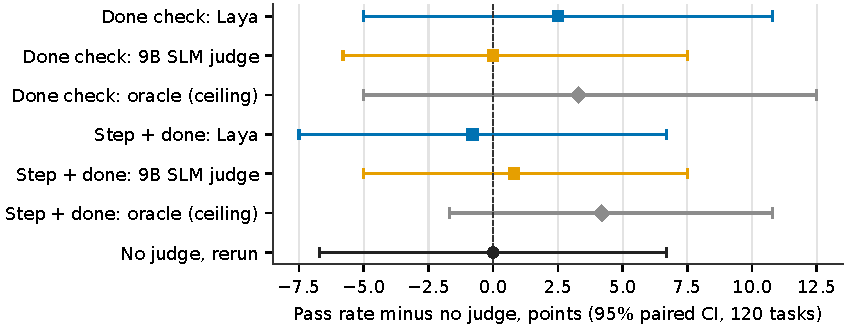
\includegraphics[width=0.74\linewidth]{figs/fig5_live.pdf}
\caption{Live runs on the 120 validation tasks: pass rate minus no judge, with 95\% paired confidence intervals.}\label{fig:live}
\end{figure}

\begin{table}[H]
\centering\tablestyle
\caption{Live results on the 120 validation tasks.}\label{tab:live}
\begin{tabularx}{\linewidth}{Yrlrr}
\toprule
\rowcolor{white}\textbf{System} & \textbf{Pass} & \textbf{vs no judge [95\% CI]} & \textbf{Judge tok. / task} & \textbf{s / task} \\
\midrule
No judge & 43.3\% & & 0 & 207 \\
Done check: \textbf{Laya} & \textbf{45.8\%} & \textbf{+2.5 [$-$5.0, +10.8]} & $\approx$0 & 234 \\
Done check: 9B SLM judge & 43.3\% & +0.0 [$-$5.8, +7.5] & 10,334 & 454 \\
Done check: oracle & 46.7\% & +3.3 [$-$5.0, +12.5] & 0 & 235 \\
Step and done checks: Laya & 42.5\% & $-$0.8 [$-$7.5, +6.7] & $\approx$0 & \\
Step and done checks: 9B SLM judge & 44.2\% & +0.8 [$-$5.0, +7.5] & & \\
Step and done checks: oracle & 47.5\% & +4.2 [$-$1.7, +10.8] & 0 & \\
\bottomrule
\end{tabularx}
\end{table}

\begin{itemize}
  \item \textbf{The Laya done check scores 2.5 points higher than the SLM-judge done check} (not significant), at about zero judge tokens and half the time per task.
  \item \textbf{No live difference is significant.} Two identical no-judge runs disagree on 28 of 120 tasks.
  \item \textbf{There is little room on this agent.} A perfect checker adds only +4.2, against +9.2 on the weaker Qwen3.5 4B agent. A live gain therefore needs more seeds or a weaker agent.
\end{itemize}

\subsection{Primary metric on validation}
\begin{table}[H]
\centering\tablestyle
\caption{Primary metric on validation: finetuned Laya against the 9B SLM judge, scored against the guide v2 annotations. CIs: paired bootstrap over scenarios. The primary column uses the proposal's mapping (Laya's ``not done'' counts as a false claim). The closing-message off-track column instead counts ``not done'' as off track; under that mapping the primary is +2.7 to +4.3, with CIs that include zero.}\label{tab:primary}
\begin{tabularx}{\linewidth}{P{0.13\linewidth}YYYY}
\toprule
\rowcolor{white}\textbf{Labels} & \textbf{Off track, calls} (Laya / 9B) & \textbf{Off track, closing msgs} (Laya / 9B) & \textbf{False claim} (Laya / 9B, positives) & \textbf{Primary,} Laya $-$ 9B [95\% CI] \\
\midrule
Swayam (A) & 0.42 / 0.34 & 0.52 / 0.34 & 0.07 / 0.05 (15) & $-$1.0 [$-$7.3, +3.2] \\
Aaditya (B) & 0.36 / 0.29 & 0.42 / 0.28 & 0.10 / 0.05 (10) & +2.0 [$-$5.4, +7.1] \\
Both agree & 0.39 / 0.29 & 0.47 / 0.34 & 0.07 / 0.06 (6) & +0.5 [$-$6.7, +5.1] \\
\bottomrule
\end{tabularx}
\end{table}

\begin{itemize}
  \item \textbf{Off track:} Laya leads by 7 to 18 F1 points. On closing messages, against Swayam's annotations, the interval is above zero: +18.0 [+3.3, +32.2].
  \item \textbf{False claim:} a tie near zero, on only 6 to 15 positives, because Laya has no false-claim head yet.
  \item \textbf{The primary hypothesis is therefore neither met nor falsified on validation.} Section~\ref{sec:challenges} gives the fix.
\end{itemize}

% =====================================================================
\section{Ablations}\label{sec:ablations}
\begin{table}[H]
\centering\tablestyle
\caption{Ablations run so far. The first three are the deeper ablations the TA asked for.}\label{tab:ablations}
\begin{tabularx}{\linewidth}{P{0.24\linewidth}Y}
\toprule
\rowcolor{white}\textbf{Ablation} & \textbf{Result} \\
\midrule
\textbf{Correction action} (Qwen3 8B, validation) & \textbf{Block and warn does not help even with a perfect judge} (oracle +2.5 [$-$1.7, +6.7]) and hurts with the SLM judge (18.3\% against 25.8\% for no judge). Rollback removes that damage (22.5 to 24.2\%). A vote of 3 with the SLM judge gives nothing (20.8\%). \textbf{Rollback plus the done check is the only lever that moved results:} the oracle gains +5.8 [0.0, +12.5] on Qwen3 8B and +9.2 [+2.5, +15.8] on Qwen3.5 4B. \\
\textbf{Finetuning gain per question} & Done check: AUROC 0.53 as is, 0.59 head only, 0.79 full finetune. Step check: AUROC 0.57 as is against 0.90 finetuned (2,427 pooled validation calls). \\
\textbf{Per question against rules} & Rules score a primary F1 of 0.10 to 0.11 and off-track F1 0.17 to 0.19 (Table~\ref{tab:offline}). Finetuned Laya reaches 0.36 to 0.42 off-track F1 on calls (Table~\ref{tab:primary}; the step sets differ slightly). On false claims both are near zero (rules 0.00 to 0.05, Laya 0.07 to 0.10). \\
\textbf{Agent model and reasoning} & Qwen3 8B 25.8\%, Qwen3.5 4B 40.0\%, Qwen3.5 9B 43.3\%. Reasoning on is 6.6 points lower and 2.5$\times$ slower. \\
\textbf{Input format, Laya as is} & 4 state formats and 8 question wordings: AUROC 0.39 to 0.67. Putting the step first fixes the truncation but adds no signal. \\
\textbf{How the done head is used} & As a gate on every closing message: 37.5\%. Only for the done check: 42.5\%. \\
\textbf{SLM judge prompt} & Against Swayam's (A) labels, the harness judge prompt raises the 9B's call F1 from 0.28 to 0.34, which shrinks Laya's lead on calls from +14.5 to +8.2 points. \\
\textbf{Annotation guide version} & Over 200 steps, agreement with the checkers rises from kappa 0.53 to 0.87 for Swayam, and from 0.62 to 0.71 for Aaditya (Section~\ref{sec:annot}). \\
\bottomrule
\end{tabularx}
\end{table}

\textbf{Planned for the final submission} (all offline and cheap):
\begin{itemize}
  \item \textbf{State parts.} Drop the plan, the recent calls or the evidence list from Laya's input, and measure the effect on off-track detection. This tests our core state design, as the TA asked.
  \item \textbf{Escalation budget.} Send 0, 10, 20, 30 or 100\% of uncertain steps to the SLM judge, and plot F1 against judge tokens.
  \item \textbf{Seeds.} Run three seeds for every finetune.
  \item \textbf{Question order.} Compare feeding the Q1 answer to Q2 with leaving it out.
\end{itemize}

% =====================================================================
\section{Annotation quality check}\label{sec:annot}
The revised proposal requires the annotation to be checked on a stratified sample, half flagged by the annotators and half not:
\begin{itemize}
  \item \textbf{Checkers:} Pavan and Shuban each labelled every sampled step blind, then settled their disagreements together. They saw neither the annotations nor the oracle labels.
  \item \textbf{Sample:} two rounds of 100 validation steps, each with 50 calls and 50 turn ends.
  \item \textbf{Reweighting:} kappa is reweighted to the real mix of steps.
  \item \textbf{Decision rule:} below 0.6, rewrite the guide; between 0.6 and 0.8, label more steps. The pass bar is 0.7.
\end{itemize}

\begin{figure}[H]
\centering
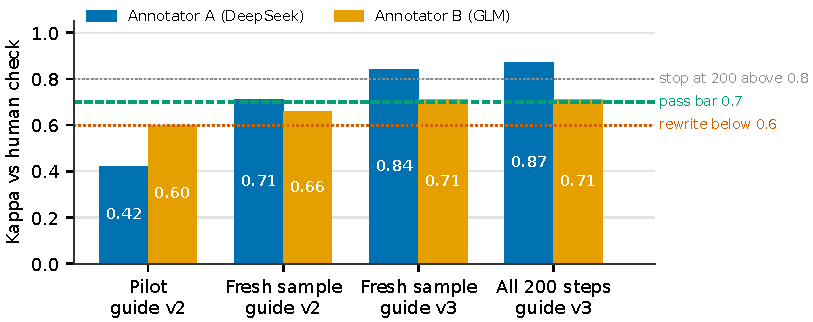
\includegraphics[width=0.76\linewidth]{figs/fig6_agreement.pdf}
\caption{Annotation agreement with the checkers' consensus (Cohen's kappa, reweighted to the real mix of steps).}\label{fig:agreement}
\end{figure}

\begin{table}[H]
\centering\tablestyle
\caption{Annotation check results (kappa, reweighted; every step, problem vs fine).}\label{tab:agreement}
\begin{tabularx}{\linewidth}{Ycccp{0.2\linewidth}}
\toprule
\rowcolor{white}\textbf{Round} & \textbf{Checker vs checker} & \textbf{vs Swayam (A)} & \textbf{vs Aaditya (B)} & \textbf{Decision} \\
\midrule
Pilot, guide v2 & 0.89 & 0.42 & 0.60 & below 0.6: rewrite the guide \\
Fresh sample, guide v2 & 0.87 & 0.71 & 0.66 & \\
Fresh sample, guide v3 (fair test) & 0.87 & \textbf{0.84} & \textbf{0.71} & passes 0.7 \\
All 200 steps, guide v3 & & \textbf{0.87} & \textbf{0.71} & passes 0.7 \\
\bottomrule
\end{tabularx}
\end{table}

\textbf{What guide v3 changed.}
\begin{itemize}
  \item \textbf{Done means every part.} Split the request into its parts; a turn is done only if every part has a successful call behind it.
  \item \textbf{Plans do not authorise changes.} A change listed in the plan but not asked for in the request is still unrequested.
  \item \textbf{Steps toward the goal are on track,} such as copying a file before renaming it.
  \item \textbf{Self-chosen values need asking.} If the agent picks a name for a change itself, it should have asked the user.
  \item \textbf{The evidence list is trusted.}
\end{itemize}

The fresh sample was drawn after v3 was written, so it is the fair test. Under the proposal's rule, the result is in the ``label more steps'' band, and the next 100 check steps come from the test runs. The weakest class left is false claims at turn ends, at kappa 0.38 to 0.46 on few positives.

% =====================================================================
\section{Worked example of a failure}
\textbf{Task} \code{multi\_turn\_base\_93} (car domain, validation, failed).
\begin{enumerate}[leftmargin=16pt]
  \item \textbf{``How much fuel do I have?''} One correct call. Done.
  \item \textbf{``Fill it to full, start the engine with START, check the tire pressure.''}
  \begin{itemize}
    \item \textbf{What the agent did:} filled 50 litres (error: over capacity), tried to start the engine (error: the doors must be locked, naming them), checked the tire pressure, then reported what it could not do.
    \item \textbf{What it missed:} locking the doors and pressing the brake, though the error message named the fix.
    \item \textbf{Pattern:} stopped early, an easy catch for a done check.
  \end{itemize}
  \item \textbf{``If tire pressure is below 40 psi, give me directions to the nearest tire shop.''}
  \begin{itemize}
    \item \textbf{What the agent did:} found the shop and told the user the address.
    \item \textbf{What it missed:} it never set the navigation.
    \item \textbf{Pattern:} the agent is confident, and ``directions'' has to be read as an action. Subtle cases like this are where an SLM judge with reasoning may still beat a 0.4B classifier. That is why the proposal keeps escalation to the SLM judge for uncertain steps.
  \end{itemize}
\end{enumerate}
No call in this task was harmful. Both failures are omissions, which a judge that only sees proposed steps cannot see.

% =====================================================================
\section{Challenges and mitigation}\label{sec:challenges}
\begin{table}[H]
\centering\tablestyle
\caption{Challenges met so far and how we address them.}\label{tab:challenges}
\begin{tabularx}{\linewidth}{P{0.38\linewidth}Y}
\toprule
\rowcolor{white}\textbf{Challenge} & \textbf{Mitigation} \\
\midrule
\textbf{False claims are rare:} 6 to 15 on validation, while the primary metric needs about 300; Laya also has no false-claim head yet. & Run test passes until 300 false claims or 8 passes, decided before seeing any test result. Train a typed closing-message head. Plan to create training false claims by editing passed traces so their last needed call fails, which replay confirms. \\
\textbf{The oracle's off-track label disagrees with the annotators} (kappa 0.04 to 0.15). & Replace it with narrower step labels: unneeded irreversible call, made-up value, breaks the task. Score against the checked annotations. \\
\textbf{Annotators disagreed on turn ends} (kappa 0.54 under guide v1, 0.61 under v2). & Ran the 200-step check and rewrote the guide (v3). Agreement now passes 0.7. \\
\textbf{Laya as is is unusable:} it blocks 87.6\% of steps and truncates the step it judges. & Step first in the state, and a full finetune: AUROC 0.91 on calls. \\
\textbf{A step judge cannot see omissions,} which are about half of all failures. & Added the done check at turn end, and rollback in place of block and warn. \\
\textbf{Little room on the 9B agent, and a noisy pass rate:} oracle +4.2; 28 of 120 tasks flip between identical runs. & Three seeds per system, and a pilot on the weaker 4B agent (oracle +9.2). Report the per-step F1 claim separately from task accuracy. \\
\textbf{A threshold chosen on 50 dev positives overfit:} F1 0.36, against 0.53 at 0.5. & Choose thresholds by grouped cross-validation on train. \\
\textbf{Compute:} the 2080 Ti cards on Ada are slow, Granite timed out, and a 32B model needs 4 cards. & Moved the 9B runs to a 48 GB RTX 6000 Ada on Turing, scored Granite on CPU, and dropped the 32B directed runs. \\
\textbf{BFCL quality:} unsound answer keys, and the turn where the agent should ask is never scored. & Use the cleaned split and the empty-turn check; we plan to also report act-or-ask decision accuracy. \\
\bottomrule
\end{tabularx}
\end{table}

% =====================================================================
\section{Changes from the proposal}\label{sec:changes}
\begin{itemize}
  \item \textbf{Agent model.} Qwen3.5 9B replaces Qwen3 8B (43.3\% against 25.8\% on validation). Qwen3 8B remains the agent of the test-set baselines (Table~\ref{tab:test}).
  \item \textbf{Directed runs dropped.} The directed runs with a large model (Qwen3 32B in proposal v5) cost too many GPU-hours for the gain. The step head trains on pooled natural mistakes from two agent models, Qwen3.5 9B and Qwen3 8B. False-claim examples are planned to come from edited traces.
  \item \textbf{Natural training runs.} The planned Qwen3 8B (3 passes) and Qwen3 4B (1 pass) became one pass of the 9B over the 888 train tasks, plus the recorded Qwen3 8B steps.
  \item \textbf{Correction actions.} Block plus a fixed warning and a fresh doer became rollback-and-resample plus the done check, because block and warn did not help (Section~\ref{sec:ablations}).
  \item \textbf{Offline reference judge.} Qwen3 14B became Gemma 4 12B, a different model family from the agent.
  \item \textbf{Hardware.} The 9B runs and the Laya finetunes moved from the Ada 2080 Ti cards to a 48 GB RTX 6000 Ada on Turing.
  \item \textbf{A fourth question.} The done check at turn end (done or not done; a typed version is planned) covers the half of failures that a step judge cannot see.
  \item \textbf{Q3 folded in.} The unneeded-irreversible-call question is now one of the ``bad step'' labels of the step head.
  \item \textbf{Labelling.} Two annotators label every step, and two checkers label a stratified 200-step sample to measure the annotators' quality, with the decision rule of Section~\ref{sec:annot}. This replaces hand-labelling 2,000 to 3,000 test steps directly with a fifth labelled twice.
\end{itemize}

% =====================================================================
\section{Timeline to the final submission}
\begin{figure}[H]
\centering
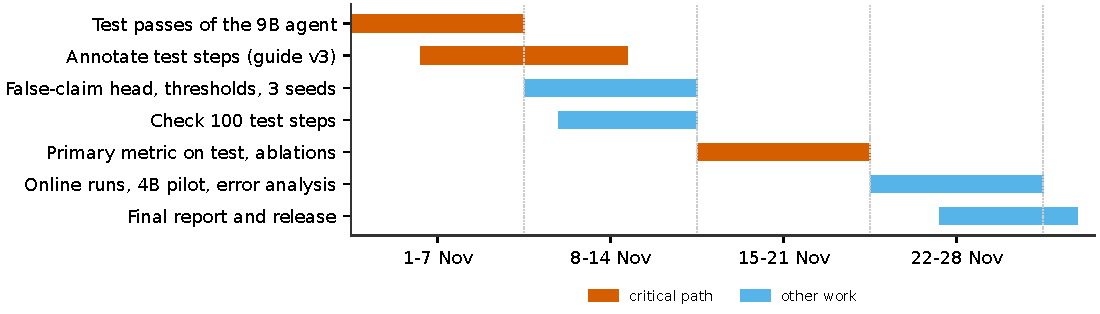
\includegraphics[width=0.9\linewidth]{figs/fig7_timeline.pdf}
\caption{Plan to the final submission (weeks of November 2026).}\label{fig:timeline}
\end{figure}

\begin{table}[H]
\centering\tablestyle
\caption{Work plan and owners.}\label{tab:timeline}
\begin{tabularx}{\linewidth}{P{0.13\linewidth}YP{0.2\linewidth}}
\toprule
\rowcolor{white}\textbf{Week} & \textbf{Work} & \textbf{Owner} \\
\midrule
1--7 Nov & Test passes of the 9B agent (about 0.5 GPU-hour each) until 300 false claims; annotate the test steps with guide v3. & Pavan, Swayam, Aaditya \\
8--14 Nov & Typed closing-message head with a false-claim class; thresholds by grouped cross-validation; 3 seeds; check 100 test steps. & Pavan, Shuban \\
15--21 Nov & Primary metric on test with paired bootstrap CIs and Holm correction; state-part and escalation-budget ablations; cost per judge. & Shuban, Swayam \\
22--28 Nov & Online test runs (no judge, Laya, SLM judge, oracle) with rollback and the done check; 4B pilot; error analysis of every miss and false alarm. & Pavan, Aaditya \\
By the deadline & Final report, release of the checked annotations, repository clean-up. & Everyone \\
\bottomrule
\end{tabularx}
\end{table}

Dates shift with the final deadline. The critical path is the test passes, then the test annotation, then the offline test evaluation.

% =====================================================================
\section{Repository and reproduction}
\textbf{Repository:} \url{https://github.com/ch-pavan/lma-grp-project/tree/main}

\begin{table}[H]
\centering\tablestyle
\caption{Repository layout.}\label{tab:repo}
\begin{tabularx}{\linewidth}{P{0.27\linewidth}Y}
\toprule
\rowcolor{white}\textbf{Path} & \textbf{Contents} \\
\midrule
\code{proposal/} & Proposal source, figures and PDF \\
\code{shuban\_findings/} & Harness code (\code{code/}), Ada job scripts, test baselines, correction modes, off-the-shelf judges, Qwen3 8B finetune data \\
\code{analysis/} & Oracle and step labels, annotation scripts, Laya finetuning and evaluation, primary metric, write-ups \\
\code{human\_check/} & Annotation guides v2 and v3, the two check samples, checkers' sheets and results \\
\code{runs/raw/}, \code{runs/data/} & Run outputs, labels, annotations and Laya datasets \\
\code{runs/turing/} & Job scripts for the 9B runs and Laya finetunes \\
\code{mid\_submission/} & This report (LaTeX source), its figures and the build scripts \\
\bottomrule
\end{tabularx}
\end{table}

\begin{tcolorbox}[colback=shade,colframe=rule,boxrule=0.4pt,arc=1pt,left=6pt,right=6pt,top=3pt,bottom=3pt,fontupper=\small\ttfamily]
sh runs/unpack\_data.sh \hfill\textrm{\itshape rebuild runs/data from the repository}\\
python analysis/primary\_val.py \hfill\textrm{\itshape primary metric on validation}\\
python human\_check/score.py human\_check/val2 -{}-guide v3 \hfill\textrm{\itshape annotation check, fresh sample}\\
python mid\_submission/make\_figs.py \hfill\textrm{\itshape redraw the figures}\\
python mid\_submission/build\_report.py \hfill\textrm{\itshape rebuild this PDF}
\end{tcolorbox}

\end{document}
